

\msection{Defensive Diversification: Speculative Side-channel protection}

As previously discussed in \autoref{background:wasm:ecosystems}, \Wasm is rapidly gaining traction in backend environments. 
Companies like Cloudflare and Fastly are encouraging the use of \Wasm in their edge computing platforms, allowing developers to deploy faster applications in a modular and securely sandboxed fashion. 
Typically, these client \Wasm applications are designed as isolated services with a single, focused responsibility.
This model is usually called Function-as-a-Service (FaaS) \cite{pMendkiServerless, 1244493Jacobsson}.
In \autoref{fig:edge_model} we illustrate how \Wasm binaries are used in FaaS platforms.
Developers can submit any \Wasm binary to the FaaS platform that are then replicated and moved around the Edge-cloud worldwide platform.

\todo{Align the figure with the terms}

\begin{figure}[h]
    \centering
    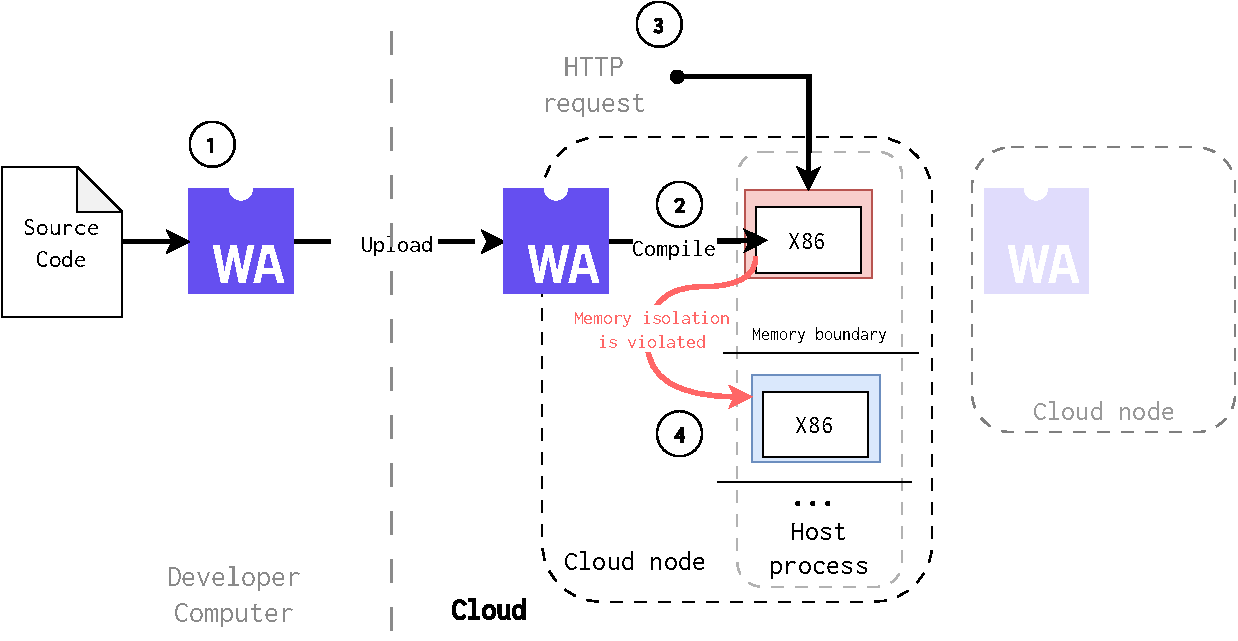
\includegraphics[width=0.8\linewidth]{figures/edge.pdf}
    \caption{\Wasm binaries on FaaS platforms.}
    \label{fig:edge_model}
\end{figure}

The core concept behind \wasm in FaaS platforms is the ability to host thousands of client \Wasm binaries within a single host process, which is then distributed across multiple servers and data centers. 
To achieve this, the platforms compile the \wasm programs to native code, which is then executed in a sandboxed environment.
Then, the host processes are capable of instantiating a new Wasm sandbox for each client function, executing it in response to individual user requests in a matter of nanoseconds. 
Utilizing \Wasm enables these platforms to inherently isolate the execution of client functions from one another as well as from the host process.
However, this isolation is not foolproof against Spectre attacks \cite{Spectre,Narayan2021Swivel}.


In the subsequent sections, we illustrate how diversification can be used to protect \Wasm binaries against Spectre attacks.
We show a case of Defensive Software Diversification for the sake of protecting \Wasm binaries. 

\msubsection{Threat model: speculative side-channel attacks}

Let us illustrate the threat model in which a \Wasm program could be susceptible in FaaS platforms.
Developers can submit any \Wasm binary to the FaaS platform.
This includes potential malicious actors that could upload a \wasm binary that, when compiled to native code, uses Spectre attacks to leak sensitive information from the host process.
Spectre attacks exploit hardware predictors to induce misspredictions and speculatively execute instructions—gadgets that would not run sequentially. 
The attacker could then use this information to infer the contents of the memory of other client functions, or even the host process itself.

Narayan and colleagues \cite{Narayan2021Swivel} dissected the possible Spectre attacks for \wasm binaries into three categories based on the specific hardware predictor that is exploited and the specific FaaS scenario: Sandbox breakout attacks, Sandbox poisoning attacks and Host poisoning attacks.
The first one, exploits the branch target buffer by predicting the target of an indirect jump, thereby rerouting speculative control flow to an arbitrary target.
The second one takes advantage of the pattern history table to anticipate the direction of a conditional branch during the ongoing evaluation of a condition.
The third and last one exploits the return stack buffer that stores the locations of recently executed call instructions to predict the target of \texttt{ret} instructions. 
Each attack methodology relies on the extraction of memory bytes from another hosted \wasm binary that executes in the same host process.



\todo{Add diagram}
\todo{Explain here the threat model with the diagram}

%\lipsum[1]

%\lipsum[1]

\msubsection{Approach}
%\lipsum[1]

- Use of wasm-mutate

\msubsection{Results}

- Diminshing of BER
- Rockiki paper on portable side channel in browsers.



\todo{TBD discuss deoptimization}
% \subsection{Deoptimization}

\subsection{Partial input/output validation}

% We need to talk about this because, we do this checking right noe and it is probably a reason for the low count of variants.
When \tool generates a variant, it can be executed to check the input/output equivalence.
If the variant has a \_start function, both binaries, the original and the variant can be initialized. 
If the state of the memory, the globals and the stack is the same after executing the \_start function, they are partially equivalent.
%This mechanismm is already implemented in the fuzzing campaign of wasmtime.

The \_start function is easier to execute given its signature.
It does not receive parameters.
Therefore, it can be executed directly.
Yet, since a \Wasm program might contain more than one function that could be indistinctly called with and arbitrary number of parameters, we are not able to validate the whole program.
Thus, we call the checking of the initialization of a \wasm variant, a partial validation.

\subsection{Some other works to be cited along with the paper. Mostly in the Intro}

\emph{Spectre and side-channel defenses}

- paper 2021: Read this, since it is super related, \url{https://www.isecure-journal.com/article_136367_a3948a522c7c59c65b65fa87571fde7b.pdf} \cite{WasmSpectre}


- A dataset of Wasm programs: \cite{nicholson2023wasmizer}

- Papers 2020

- Papers 2019
- \cite{10.1145/3510003.3510070}

Selwasm: A code protection mechanism for webassembly


Babble

- https://arxiv.org/pdf/2212.04596.pdf

Principled Composition of Function Variants for Dynamic
Software Diversity and Program Protection

- https://dl.acm.org/doi/10.1145/3551349.3559553

How Far We’ve Come – A Characterization Study of Standalone WebAssembly Runtimes

- https://ieeexplore.ieee.org/document/9975423

Code obfuscation against symbolic execution attacks

Code artificiality: A metric for the code stealth based on an n-gram model

Semantics-aware obfuscation scheme prediction for binary

Wobfuscator: Obfuscating javascript malware via opportunistic translation to webassembly

Synthesizing Instruction Selection Rewrite Rules from RTL using SMT
"We also synthesize integer rewrite rules from WebAssembly to RISC-V "

Wafl: Binary-only webassembly fuzzing with fast snapshots



\begin{tcolorbox}[title=Contribution paper,boxrule=1pt,arc=.2em,boxsep=1.0mm]
    The case discussed in this section is fully detailed in Cabrera-Arteaga \etal "WASM-MUTATE: Fast and Effective Binary Diversification for WebAssembly"
    \emph{Under review}
    \url{https://arxiv.org/pdf/2309.07638.pdf}. 
\end{tcolorbox}



